\chapter{Analysis and Results}
In this chapter the analysis and the result of the research findings will be presented. The overall structure will follow the structure of the chapter Methodology to easier correlate method used and the presented analysis. 

\begin{figure}[H]
    \centering
    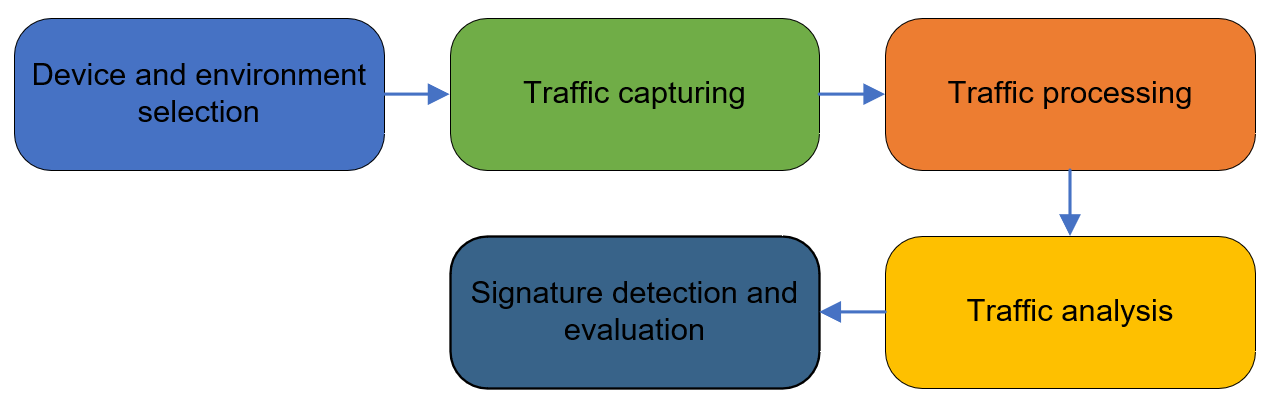
\includegraphics[width=\textwidth]{figures/AnalysisFlow.png}
    \caption{Analysis Flow}
    \label{fig:AnalysisFlow}
\end{figure}

\section{Device and environment selection}
Irobot Roomba i7 was selected as the preferred robot vacuum cleaner in this research, in the corresponding section in chapter Method. In this section the rest of the devices in the smart home environment will be presented. 

\paragraph{Capturing platfrom}
Capturing platform is chosen to be a Raspberry PI 3b+, loaded with Kali Linux operation system. The reason for this is the availability. The author of this thesis had available raspberry PIs through his work. Kali Lunux is open source and have deigned versions to run on Raspberry PI. The OS also includes the analysis tools Wireshark and Tshark that is required in this research. 
An external Wi-Fi adapter is added to the Raspberry PI, this was recommended by \cite{wifi_adapter_monitor_mode}. This also allows data to be extracted from the capturing platform via ftp services on the build in wi-fi network interface card.

\begin{itemize}
    \item wlan0, is buildt in wi-fi interface card
    \item wlan1, is the external TP-LINK TL-WN722N V2 adapter
    \item eth0, is the buldt in ethernet IEEE 802.3 interface card
\end{itemize}

\begin{table}[H]
\centering
\caption{Capturing platform specifications}
\label{tab:CapturingPlatfromSpec}
\begin{tabular}{|ll|}
\hline
\multicolumn{2}{|c|}{\textbf{Capturing platform}}                         \\ \hline
\multicolumn{1}{|l|}{Hardware}               & Raspberry Pi 3b+           \\ \hline
\multicolumn{1}{|l|}{Software}               & Kali Linux                 \\ \hline
\multicolumn{1}{|l|}{Tshark}                 & Version                    \\ \hline
\multicolumn{1}{|l|}{External wi-fi adapter} & TP-LINK TL-WN722N V2       \\ \hline
\multicolumn{1}{|l|}{External storage}       & Micro SD card SanDisk 32GB \\ \hline
\end{tabular}
\end{table}

\paragraph{Analysis platform}
HP Elitebook with windows 11 is used abs the analysis platform, the reason is the availability of the machine. It is installed with Wireshark, Tshark and VS code. 

\begin{table}[H]
\centering
\caption{Analysis platform specifications}
\label{tab:AnalysisPlatfromSpec}
\begin{tabular}{|ll|}
\hline
\multicolumn{2}{|c|}{\textbf{Analysis platform}}      \\ \hline
\multicolumn{1}{|l|}{Hardware}  & HP Elitebook        \\ \hline
\multicolumn{1}{|l|}{Software}  & Windows 11          \\ \hline
\multicolumn{1}{|l|}{Wireshark} & 4.0.2               \\ \hline
\multicolumn{1}{|l|}{VS code}   & 1.77.3 (user setup) \\ \hline
\end{tabular}
\end{table}

\paragraph{Access point}
TP-Link Archer MR200 is acuired, this access point have LAN ports to connect towards the ISP router and wireless capabilities. It can separate connected WLAN and LAN with the use of Network address translation. 

\begin{table}[H]
\centering
\caption{Access point specifications}
\label{tab:AccessPointSpec}
\begin{tabular}{|ll|}
\hline
\multicolumn{2}{|c|}{\textbf{Access Point}}                        \\ \hline
\multicolumn{1}{|l|}{Hardware} & TP-Link archer MR200(EU) ver:5.30 \\ \hline
\multicolumn{1}{|l|}{Software} & version                           \\ \hline
\end{tabular}
\end{table}

\paragraph{LAN Switch}
A Cisco Catalyst 2960 series switch is used, this due to the support for SPAN port configuration. 

\begin{table}[H]
\centering
\caption{LAN Switch specifications}
\label{tab:LanSwitchSpec}
\begin{tabular}{|ll|}
\hline
\multicolumn{2}{|c|}{\textbf{LAN Switch}}                           \\ \hline
\multicolumn{1}{|l|}{Hardware} & Cisco Catalyst 2960 series, 8 port \\ \hline
\multicolumn{1}{|l|}{Software} & ISO 12.2(35)SE5                    \\ \hline
\end{tabular}
\end{table}


\subsection{Smart Home environment}
All these devices connected will create the WLAN/LAN which is used in all environments through this research. The only change will be the Internet delivered by the ISP, if not local configuration and impact is not taken into account this could weekend the reliability of the result. Optimal there would be a completely different smart home infrastructure, but due to limited resources and time it was done with the same internal smart home network. The complete overview is illustrated in \ref{fig:SmartHomeSetup} 

\begin{figure}[H]
    \centering
    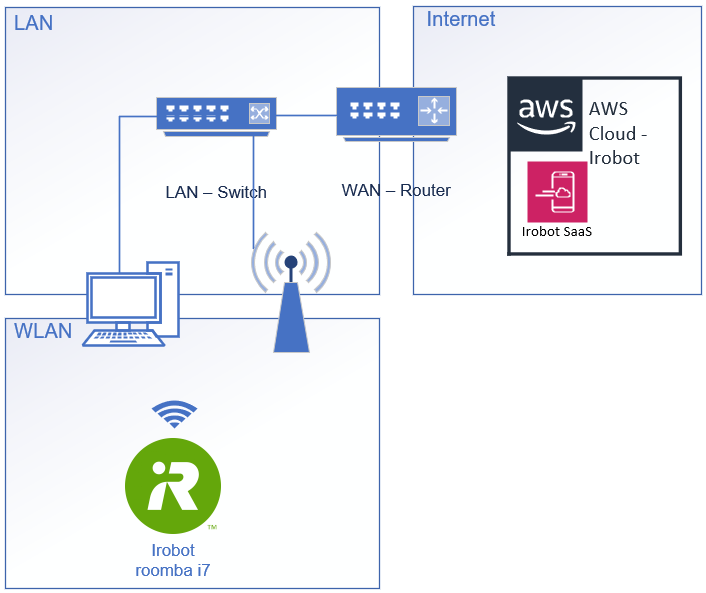
\includegraphics[width=\textwidth]{figures/SmartHomeSetup.png}
    \caption{SmartHomeSetup}
    \label{fig:SmartHomeSetup}
\end{figure}


\section{Event selection}
In this section all the different event will be presented. These are based on different features for the Irobot Roomba i7 vacuum cleaner. The selected events are: 

\begin{itemize}
    \item \textbf{Standby event}, the vacuum cleaner is connected, but not interacted with. This will be used to identify standby traffic which can be filtered out for the events. 
    \item \textbf{Scheduled cleaning}, users can configure scheduled cleaning jobs based on time and date. The vacuum cleaner will then start cleaning at the configured time. This could potentially expose some parts of the daily routine.
    \item \textbf{Automated cleaning}, used integrated services such as location, smart lock and smart garage port to trigger events. For this research location integration with IFFF will be used to trigger the cleaning. If this could be identified, it could with high confidence say that the home owner left the resident.
    \item \textbf{Application triggered cleaning}, user opens the Irobot application and manually triggers a cleaning job. Identification will show human interaction.
    \item \textbf{Physical triggered cleaning}, user push a physical button on the vacuum cleaner to trigger cleaning. This would tell if the user is home. 
    \item \textbf{Application start}, user starts the application on their phone. This will expose user interaction. 
    \item \textbf{Bin remove}, user eject the bin and reenters it. this is the normal procedure when it is full. It can expose that user is home. 
\end{itemize}

\subsection{Event description}

\begin{figure}[H]
    \centering
    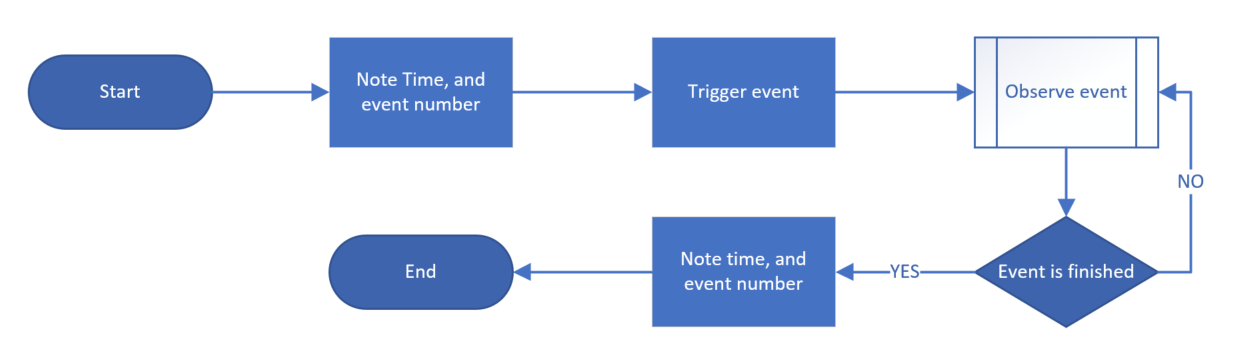
\includegraphics[width=\textwidth]{figures/EventTriggeringProcess.png}
    \caption{Capturing process}
    \label{fig:EventTriggeringProcess}
\end{figure}

\subsection{Event tests}
In this section all the different test flows will be described. This will make the tests and results more reproducible. 

\subsubsection{Standby Traffic}
This test is executed to identify network traffic generated to the robot vacuum cleaner in a standby mode. This means that there is no interaction done by human. 

\begin{itemize}
    \item \textbf{Event flow} \begin{enumerate}
                                    \item Start captuing of LAN and WLAN traffic
                                    \item Wait 14 days without any human interaction
                                    \item Stop capturing
                                \end{enumerate}
    \item \textbf{Number of events:} 1
\end{itemize}

\subsubsection{Scheduled Cleaning}
Scheduled cleaning can be configured through the application. Users can schedule a cleaning, specifying area in the smart home, time which the cleaning should start, as well as how often this should occur. 
\begin{itemize}
    \item \textbf{Event flow} \begin{enumerate}
                                    \item Schedule cleaning outside of event capture
                                    \item Note the time when cleaning started
                                    \item Note when "finished cleaning" notification is received
                                \end{enumerate}
    \item \textbf{Number of events in each environment:} 10
\end{itemize}

\subsubsection{Automated cleaning}
Irobot has features to integrate other services as triggers for events. This includes IFFF location tracker, Agust smart lock system, ecobee termotat system, My Leviton smart home integration and MyQ garage system. In this research the IFFF location system will be used. Cleaning is then triggered when the users phone is x meters away from home, where x is between 100m and 1 km. 

\begin{itemize}
    \item \textbf{Event flow} \begin{enumerate}
                                    \item Configure automated cleaning outside of event capture
                                    \item Leave the smart home environment
                                    \item Note when cleaning notification is received
                                    \item Note when "finished cleaning" notification is received
                                \end{enumerate}
    \item \textbf{Number of events in each environment:} 10
\end{itemize}

\subsubsection{Application triggered cleaning}
In the application users can trigger cleaning. There is a predefined "clean all" option, if the user have not customized. Cleaning is triggered when the user is pressing a cleaning option in the application.

\begin{itemize}
    \item \textbf{Event flow} \begin{enumerate}
                                    \item Note time
                                    \item Open the application and trigger "clean all" event
                                    \item Note when "finished cleaning" notification is received
                                \end{enumerate}
    \item \textbf{Number of events in each environment:} 10
\end{itemize}

\subsubsection{Physical triggered cleaning}
The Irobot roomba i7 has a physical cleaning button on top of the vacuum cleaner. A "clean all" vent is triggered when this button is pressed.

\begin{itemize}
    \item \textbf{Event flow} \begin{enumerate}
                                    \item Note time
                                    \item Press the physical clean button on the vacuum cleaner
                                    \item Note when "finished cleaning" notification is received
                                \end{enumerate}
    \item \textbf{Number of events in each environment:} 10
\end{itemize}

\subsubsection{Open application}
When the application is opened information will be displayed, through the application the user can interact and change setting. 

\begin{itemize}
    \item \textbf{Event flow} \begin{enumerate}
                                    \item Note time
                                    \item Open the application on the smart phone
                                    \item wait for some time
                                    \item Close application
                                    \item Note time
                                \end{enumerate}
    \item \textbf{Number of events in each environment:} 10
\end{itemize}

\subsubsection{Remove bin}
The Irobot roomba i7 has it own bin where dust is collected during clean. This can be removed if it is to be empty. The user will then have to physically remove and insert again. 

\begin{itemize}
    \item \textbf{Event flow} \begin{enumerate}
                                    \item Note time
                                    \item Remove the bin
                                    \item wait ta least 40 seconds
                                    \item Insert the bin
                                    \item Note time
                                \end{enumerate}
    \item \textbf{Number of events in each environment:} 10
\end{itemize}



\section{Traffic Capturing}
Standby traffic was captured between 8 and 22  of January, during this time period, no interaction with the vacuum cleaner was done. It was also continuously connected to the smart home SSID, so that it could receive traffic from the could services. The event traffic capturing is done is the two different environments according to the test matrices \ref{tab:TestMatrixEnv1} \ref{tab:TestMatrixEnv2}. The testing is done in testing intervals. All events was observers finished, before a new event was triggered. Capturing in Drammen was done during four days, due to limited availability of the smart home.  
\begin{table}[H]
\centering
\small
\caption{Test matrix Oslo}
\label{tab:TestMatrixEnv1}
\begin{tabular}{|lllllllllll|}
\hline
\multicolumn{11}{|c|}{\textbf{Scheduled cleaning}}                                                                                                                                                                                                                                                        \\ \hline
\multicolumn{1}{|l|}{Nr} & \multicolumn{1}{l|}{1}     & \multicolumn{1}{l|}{2}     & \multicolumn{1}{l|}{3}     & \multicolumn{1}{l|}{4}     & \multicolumn{1}{l|}{5}     & \multicolumn{1}{l|}{6}     & \multicolumn{1}{l|}{7}     & \multicolumn{1}{l|}{8}     & \multicolumn{1}{l|}{9}     & 10    \\ \hline
\multicolumn{1}{|l|}{Date}   & \multicolumn{1}{l|}{10.03} & \multicolumn{1}{l|}{10.03} & \multicolumn{1}{l|}{10.03} & \multicolumn{1}{l|}{10.03} & \multicolumn{1}{l|}{10.03} & \multicolumn{1}{l|}{10.03} & \multicolumn{1}{l|}{10.03} & \multicolumn{1}{l|}{10.03} & \multicolumn{1}{l|}{11.03} & 11.03 \\ \hline
\multicolumn{1}{|l|}{Start}  & \multicolumn{1}{l|}{10:44} & \multicolumn{1}{l|}{11:14} & \multicolumn{1}{l|}{12:14} & \multicolumn{1}{l|}{13:29} & \multicolumn{1}{l|}{14:59} & \multicolumn{1}{l|}{15:29} & \multicolumn{1}{l|}{15:54} & \multicolumn{1}{l|}{16:09} & \multicolumn{1}{l|}{10:09} & 10:29 \\ \hline
\multicolumn{1}{|l|}{End}    & \multicolumn{1}{l|}{10:54} & \multicolumn{1}{l|}{11:24} & \multicolumn{1}{l|}{12:24} & \multicolumn{1}{l|}{13:39} & \multicolumn{1}{l|}{15:09} & \multicolumn{1}{l|}{15:39} & \multicolumn{1}{l|}{16:04} & \multicolumn{1}{l|}{16:19} & \multicolumn{1}{l|}{10:19} & 10:39 \\ \hline
\multicolumn{11}{|c|}{\textbf{Application triggered cleaning}}                                                                                                                                                                                                                                            \\ \hline
\multicolumn{1}{|l|}{Nr} & \multicolumn{1}{l|}{1}     & \multicolumn{1}{l|}{2}     & \multicolumn{1}{l|}{3}     & \multicolumn{1}{l|}{4}     & \multicolumn{1}{l|}{5}     & \multicolumn{1}{l|}{6}     & \multicolumn{1}{l|}{7}     & \multicolumn{1}{l|}{8}     & \multicolumn{1}{l|}{9}     & 10    \\ \hline
\multicolumn{1}{|l|}{Date}   & \multicolumn{1}{l|}{28.02} & \multicolumn{1}{l|}{28.02} & \multicolumn{1}{l|}{01.03} & \multicolumn{1}{l|}{09.03} & \multicolumn{1}{l|}{09.03} & \multicolumn{1}{l|}{09.03} & \multicolumn{1}{l|}{09.03} & \multicolumn{1}{l|}{09.03} & \multicolumn{1}{l|}{12.03} & 12.03 \\ \hline
\multicolumn{1}{|l|}{Start}  & \multicolumn{1}{l|}{18:20} & \multicolumn{1}{l|}{18:35} & \multicolumn{1}{l|}{18:53} & \multicolumn{1}{l|}{07:44} & \multicolumn{1}{l|}{08:03} & \multicolumn{1}{l|}{08:25} & \multicolumn{1}{l|}{08:57} & \multicolumn{1}{l|}{09:18} & \multicolumn{1}{l|}{12:20} & 12:54 \\ \hline
\multicolumn{1}{|l|}{End}    & \multicolumn{1}{l|}{18:27} & \multicolumn{1}{l|}{18:42} & \multicolumn{1}{l|}{19:00} & \multicolumn{1}{l|}{07:49} & \multicolumn{1}{l|}{08:10} & \multicolumn{1}{l|}{08:31} & \multicolumn{1}{l|}{09:04} & \multicolumn{1}{l|}{09:26} & \multicolumn{1}{l|}{12:35} & 13:09 \\ \hline
\multicolumn{11}{|c|}{\textbf{Open application}}                                                                                                                                                                                                                                                          \\ \hline
\multicolumn{1}{|l|}{Nr} & \multicolumn{1}{l|}{1}     & \multicolumn{1}{l|}{2}     & \multicolumn{1}{l|}{3}     & \multicolumn{1}{l|}{4}     & \multicolumn{1}{l|}{5}     & \multicolumn{1}{l|}{6}     & \multicolumn{1}{l|}{7}     & \multicolumn{1}{l|}{8}     & \multicolumn{1}{l|}{9}     & 10    \\ \hline
\multicolumn{1}{|l|}{Date}   & \multicolumn{1}{l|}{10.03} & \multicolumn{1}{l|}{10.03} & \multicolumn{1}{l|}{10.03} & \multicolumn{1}{l|}{10.03} & \multicolumn{1}{l|}{10.03} & \multicolumn{1}{l|}{10.03} & \multicolumn{1}{l|}{10.03} & \multicolumn{1}{l|}{10.03} & \multicolumn{1}{l|}{11.03} & 11.03 \\ \hline
\multicolumn{1}{|l|}{Start}  & \multicolumn{1}{l|}{10:26} & \multicolumn{1}{l|}{11:06} & \multicolumn{1}{l|}{11:56} & \multicolumn{1}{l|}{13:22} & \multicolumn{1}{l|}{14:58} & \multicolumn{1}{l|}{15:27} & \multicolumn{1}{l|}{15:51} & \multicolumn{1}{l|}{16:07} & \multicolumn{1}{l|}{10:06} & 10:22 \\ \hline
\multicolumn{1}{|l|}{End}    & \multicolumn{1}{l|}{10:36} & \multicolumn{1}{l|}{11:16} & \multicolumn{1}{l|}{12:06} & \multicolumn{1}{l|}{13:32} & \multicolumn{1}{l|}{15:08} & \multicolumn{1}{l|}{15:37} & \multicolumn{1}{l|}{16:01} & \multicolumn{1}{l|}{16:17} & \multicolumn{1}{l|}{10:16} & 10:32 \\ \hline
\multicolumn{11}{|c|}{\textbf{Remove bin}}                                                                                                                                                                                                                                                                \\ \hline
\multicolumn{1}{|l|}{Nr} & \multicolumn{1}{l|}{1}     & \multicolumn{1}{l|}{2}     & \multicolumn{1}{l|}{3}     & \multicolumn{1}{l|}{4}     & \multicolumn{1}{l|}{5}     & \multicolumn{1}{l|}{6}     & \multicolumn{1}{l|}{7}     & \multicolumn{1}{l|}{8}     & \multicolumn{1}{l|}{9}     & 10    \\ \hline
\multicolumn{1}{|l|}{Date}   & \multicolumn{1}{l|}{11.03} & \multicolumn{1}{l|}{11.03} & \multicolumn{1}{l|}{11.03} & \multicolumn{1}{l|}{11.03} & \multicolumn{1}{l|}{11.03} & \multicolumn{1}{l|}{11.03} & \multicolumn{1}{l|}{11.03} & \multicolumn{1}{l|}{11.03} & \multicolumn{1}{l|}{11.03} & 11.03 \\ \hline
\multicolumn{1}{|l|}{Start}  & \multicolumn{1}{l|}{17:30} & \multicolumn{1}{l|}{17:35} & \multicolumn{1}{l|}{17:40} & \multicolumn{1}{l|}{17:44} & \multicolumn{1}{l|}{17:47} & \multicolumn{1}{l|}{17:49} & \multicolumn{1}{l|}{17:51} & \multicolumn{1}{l|}{17:53} & \multicolumn{1}{l|}{17:55} & 18:01 \\ \hline
\multicolumn{1}{|l|}{End}    & \multicolumn{1}{l|}{17:31} & \multicolumn{1}{l|}{17:36} & \multicolumn{1}{l|}{17:41} & \multicolumn{1}{l|}{17:45} & \multicolumn{1}{l|}{17:48} & \multicolumn{1}{l|}{17:50} & \multicolumn{1}{l|}{17:52} & \multicolumn{1}{l|}{17:54} & \multicolumn{1}{l|}{17:56} & 18:02 \\ \hline
\multicolumn{11}{|c|}{\textbf{Physical triggered cleaning}}                                                                                                                                                                                                                                               \\ \hline
\multicolumn{1}{|l|}{Nr} & \multicolumn{1}{l|}{1}     & \multicolumn{1}{l|}{2}     & \multicolumn{1}{l|}{3}     & \multicolumn{1}{l|}{4}     & \multicolumn{1}{l|}{5}     & \multicolumn{1}{l|}{6}     & \multicolumn{1}{l|}{7}     & \multicolumn{1}{l|}{8}     & \multicolumn{1}{l|}{9}     & 10    \\ \hline
\multicolumn{1}{|l|}{Date}   & \multicolumn{1}{l|}{23.02} & \multicolumn{1}{l|}{23.02} & \multicolumn{1}{l|}{23.02} & \multicolumn{1}{l|}{23.02} & \multicolumn{1}{l|}{23.02} & \multicolumn{1}{l|}{09.03} & \multicolumn{1}{l|}{09.03} & \multicolumn{1}{l|}{09.03} & \multicolumn{1}{l|}{09.03} & 09.03 \\ \hline
\multicolumn{1}{|l|}{Start}  & \multicolumn{1}{l|}{18:08} & \multicolumn{1}{l|}{18:36} & \multicolumn{1}{l|}{19:14} & \multicolumn{1}{l|}{20:13} & \multicolumn{1}{l|}{20:44} & \multicolumn{1}{l|}{09:43} & \multicolumn{1}{l|}{10:30} & \multicolumn{1}{l|}{12:32} & \multicolumn{1}{l|}{13:16} & 17:44 \\ \hline
\multicolumn{1}{|l|}{End}    & \multicolumn{1}{l|}{18:24} & \multicolumn{1}{l|}{19:05} & \multicolumn{1}{l|}{19:34} & \multicolumn{1}{l|}{20:35} & \multicolumn{1}{l|}{21:06} & \multicolumn{1}{l|}{10:02} & \multicolumn{1}{l|}{10:50} & \multicolumn{1}{l|}{12:50} & \multicolumn{1}{l|}{14:05} & 18:05 \\ \hline
\multicolumn{11}{|c|}{\textbf{Automated cleaning}}                                                                                                                                                                                                                                                        \\ \hline
\multicolumn{1}{|l|}{Nr} & \multicolumn{1}{l|}{1}     & \multicolumn{1}{l|}{2}     & \multicolumn{1}{l|}{3}     & \multicolumn{1}{l|}{4}     & \multicolumn{1}{l|}{5}     & \multicolumn{1}{l|}{6}     & \multicolumn{1}{l|}{7}     & \multicolumn{1}{l|}{8}     & \multicolumn{1}{l|}{9}     & 10    \\ \hline
\multicolumn{1}{|l|}{Date}   & \multicolumn{1}{l|}{21.02} & \multicolumn{1}{l|}{22.02} & \multicolumn{1}{l|}{23.02} & \multicolumn{1}{l|}{01.03} & \multicolumn{1}{l|}{02.03} & \multicolumn{1}{l|}{03.03} & \multicolumn{1}{l|}{06.03} & \multicolumn{1}{l|}{07.03} & \multicolumn{1}{l|}{08.03} & 09.03 \\ \hline
\multicolumn{1}{|l|}{Start}  & \multicolumn{1}{l|}{21:06} & \multicolumn{1}{l|}{07:37} & \multicolumn{1}{l|}{10:10} & \multicolumn{1}{l|}{07:42} & \multicolumn{1}{l|}{11:05} & \multicolumn{1}{l|}{07:03} & \multicolumn{1}{l|}{07:04} & \multicolumn{1}{l|}{08:42} & \multicolumn{1}{l|}{07:49} & 07:22 \\ \hline
\multicolumn{1}{|l|}{End}    & \multicolumn{1}{l|}{21:14} & \multicolumn{1}{l|}{07:45} & \multicolumn{1}{l|}{10:16} & \multicolumn{1}{l|}{07:47} & \multicolumn{1}{l|}{11:10} & \multicolumn{1}{l|}{07:08} & \multicolumn{1}{l|}{07:09} & \multicolumn{1}{l|}{08:47} & \multicolumn{1}{l|}{07:54} & 07:29 \\ \hline
\end{tabular}
\end{table}


\begin{table}[H]
\small
\centering
\caption{Test matrix Drammen}
\label{tab:TestMatrixEnv2}
\begin{tabular}{|lllllllllll|}
\hline
\multicolumn{11}{|c|}{\textbf{Scheduled cleaning}}                                                                                                                                                                                                                                                        \\ \hline
\multicolumn{1}{|l|}{Nr} & \multicolumn{1}{l|}{1}     & \multicolumn{1}{l|}{2}     & \multicolumn{1}{l|}{3}     & \multicolumn{1}{l|}{4}     & \multicolumn{1}{l|}{5}     & \multicolumn{1}{l|}{6}     & \multicolumn{1}{l|}{7}     & \multicolumn{1}{l|}{8}     & \multicolumn{1}{l|}{9}     & 10    \\ \hline
\multicolumn{1}{|l|}{Date}   & \multicolumn{1}{l|}{25.02} & \multicolumn{1}{l|}{25.02} & \multicolumn{1}{l|}{26.02} & \multicolumn{1}{l|}{26.02} & \multicolumn{1}{l|}{26.02} & \multicolumn{1}{l|}{26.02} & \multicolumn{1}{l|}{26.02} & \multicolumn{1}{l|}{26.02} & \multicolumn{1}{l|}{26.02} & 26.02 \\ \hline
\multicolumn{1}{|l|}{Start}  & \multicolumn{1}{l|}{20:30} & \multicolumn{1}{l|}{21:00} & \multicolumn{1}{l|}{11:20} & \multicolumn{1}{l|}{11:50} & \multicolumn{1}{l|}{12:20} & \multicolumn{1}{l|}{12:50} & \multicolumn{1}{l|}{13:20} & \multicolumn{1}{l|}{13:50} & \multicolumn{1}{l|}{14:20} & 15:00 \\ \hline
\multicolumn{1}{|l|}{End}    & \multicolumn{1}{l|}{20:45} & \multicolumn{1}{l|}{21:15} & \multicolumn{1}{l|}{11:35} & \multicolumn{1}{l|}{12:05} & \multicolumn{1}{l|}{12:35} & \multicolumn{1}{l|}{13:05} & \multicolumn{1}{l|}{13:35} & \multicolumn{1}{l|}{14:05} & \multicolumn{1}{l|}{14:35} & 15:15 \\ \hline
\multicolumn{11}{|c|}{\textbf{Application triggered cleaning}}                                                                                                                                                                                                                                            \\ \hline
\multicolumn{1}{|l|}{Nr} & \multicolumn{1}{l|}{1}     & \multicolumn{1}{l|}{2}     & \multicolumn{1}{l|}{3}     & \multicolumn{1}{l|}{4}     & \multicolumn{1}{l|}{5}     & \multicolumn{1}{l|}{6}     & \multicolumn{1}{l|}{7}     & \multicolumn{1}{l|}{8}     & \multicolumn{1}{l|}{9}     & 10    \\ \hline
\multicolumn{1}{|l|}{Date}   & \multicolumn{1}{l|}{25.02} & \multicolumn{1}{l|}{25.02} & \multicolumn{1}{l|}{25.02} & \multicolumn{1}{l|}{25.02} & \multicolumn{1}{l|}{25.02} & \multicolumn{1}{l|}{25.02} & \multicolumn{1}{l|}{25.02} & \multicolumn{1}{l|}{25.02} & \multicolumn{1}{l|}{25.02} & 25.02 \\ \hline
\multicolumn{1}{|l|}{Start}  & \multicolumn{1}{l|}{14:30} & \multicolumn{1}{l|}{15:00} & \multicolumn{1}{l|}{15:30} & \multicolumn{1}{l|}{16:00} & \multicolumn{1}{l|}{16:30} & \multicolumn{1}{l|}{17:00} & \multicolumn{1}{l|}{17:30} & \multicolumn{1}{l|}{19:00} & \multicolumn{1}{l|}{19:30} & 20:00 \\ \hline
\multicolumn{1}{|l|}{End}    & \multicolumn{1}{l|}{14:45} & \multicolumn{1}{l|}{15:15} & \multicolumn{1}{l|}{15:45} & \multicolumn{1}{l|}{16:15} & \multicolumn{1}{l|}{16:45} & \multicolumn{1}{l|}{17:15} & \multicolumn{1}{l|}{17:45} & \multicolumn{1}{l|}{19:15} & \multicolumn{1}{l|}{19:45} & 20:15 \\ \hline
\multicolumn{11}{|c|}{\textbf{Open application}}                                                                                                                                                                                                                                                          \\ \hline
\multicolumn{1}{|l|}{Nr} & \multicolumn{1}{l|}{1}     & \multicolumn{1}{l|}{2}     & \multicolumn{1}{l|}{3}     & \multicolumn{1}{l|}{4}     & \multicolumn{1}{l|}{5}     & \multicolumn{1}{l|}{6}     & \multicolumn{1}{l|}{7}     & \multicolumn{1}{l|}{8}     & \multicolumn{1}{l|}{9}     & 10    \\ \hline
\multicolumn{1}{|l|}{Date}   & \multicolumn{1}{l|}{25.02} & \multicolumn{1}{l|}{25.02} & \multicolumn{1}{l|}{25.02} & \multicolumn{1}{l|}{25.02} & \multicolumn{1}{l|}{26.02} & \multicolumn{1}{l|}{26.02} & \multicolumn{1}{l|}{26.02} & \multicolumn{1}{l|}{26.02} & \multicolumn{1}{l|}{26.02} & 26.02 \\ \hline
\multicolumn{1}{|l|}{Start}  & \multicolumn{1}{l|}{20:50} & \multicolumn{1}{l|}{21:20} & \multicolumn{1}{l|}{22:20} & \multicolumn{1}{l|}{22:50} & \multicolumn{1}{l|}{11:10} & \multicolumn{1}{l|}{11:40} & \multicolumn{1}{l|}{12:10} & \multicolumn{1}{l|}{12:40} & \multicolumn{1}{l|}{13:10} & 13:40 \\ \hline
\multicolumn{1}{|l|}{End}    & \multicolumn{1}{l|}{20:52} & \multicolumn{1}{l|}{21:21} & \multicolumn{1}{l|}{22:22} & \multicolumn{1}{l|}{22:52} & \multicolumn{1}{l|}{11:11} & \multicolumn{1}{l|}{11:41} & \multicolumn{1}{l|}{12:11} & \multicolumn{1}{l|}{12:41} & \multicolumn{1}{l|}{13:11} & 13:41 \\ \hline
\multicolumn{11}{|c|}{\textbf{Remove bin}}                                                                                                                                                                                                                                                                \\ \hline
\multicolumn{1}{|l|}{Nr} & \multicolumn{1}{l|}{1}     & \multicolumn{1}{l|}{2}     & \multicolumn{1}{l|}{3}     & \multicolumn{1}{l|}{4}     & \multicolumn{1}{l|}{5}     & \multicolumn{1}{l|}{6}     & \multicolumn{1}{l|}{7}     & \multicolumn{1}{l|}{8}     & \multicolumn{1}{l|}{9}     & 10    \\ \hline
\multicolumn{1}{|l|}{Date}   & \multicolumn{1}{l|}{26.02} & \multicolumn{1}{l|}{26.02} & \multicolumn{1}{l|}{26.02} & \multicolumn{1}{l|}{27.02} & \multicolumn{1}{l|}{27.02} & \multicolumn{1}{l|}{27.02} & \multicolumn{1}{l|}{27.02} & \multicolumn{1}{l|}{27.02} & \multicolumn{1}{l|}{27.02} & 27.02 \\ \hline
\multicolumn{1}{|l|}{Start}  & \multicolumn{1}{l|}{15:22} & \multicolumn{1}{l|}{15:30} & \multicolumn{1}{l|}{15:35} & \multicolumn{1}{l|}{15:05} & \multicolumn{1}{l|}{15:10} & \multicolumn{1}{l|}{15:15} & \multicolumn{1}{l|}{15:20} & \multicolumn{1}{l|}{15:25} & \multicolumn{1}{l|}{15:30} & 15:35 \\ \hline
\multicolumn{1}{|l|}{End}    & \multicolumn{1}{l|}{15:23} & \multicolumn{1}{l|}{15:31} & \multicolumn{1}{l|}{15:36} & \multicolumn{1}{l|}{15:06} & \multicolumn{1}{l|}{15:11} & \multicolumn{1}{l|}{15:16} & \multicolumn{1}{l|}{15:21} & \multicolumn{1}{l|}{15:26} & \multicolumn{1}{l|}{15:31} & 15:36 \\ \hline
\multicolumn{11}{|c|}{\textbf{Physical triggered cleaning}}                                                                                                                                                                                                                                               \\ \hline
\multicolumn{1}{|l|}{Nr} & \multicolumn{1}{l|}{1}     & \multicolumn{1}{l|}{2}     & \multicolumn{1}{l|}{3}     & \multicolumn{1}{l|}{4}     & \multicolumn{1}{l|}{5}     & \multicolumn{1}{l|}{6}     & \multicolumn{1}{l|}{7}     & \multicolumn{1}{l|}{8}     & \multicolumn{1}{l|}{9}     & 10    \\ \hline
\multicolumn{1}{|l|}{Date}   & \multicolumn{1}{l|}{25.02} & \multicolumn{1}{l|}{25.02} & \multicolumn{1}{l|}{25.02} & \multicolumn{1}{l|}{25.02} & \multicolumn{1}{l|}{25.02} & \multicolumn{1}{l|}{26.02} & \multicolumn{1}{l|}{26.02} & \multicolumn{1}{l|}{26.02} & \multicolumn{1}{l|}{26.02} & 26.02 \\ \hline
\multicolumn{1}{|l|}{Start}  & \multicolumn{1}{l|}{22:00} & \multicolumn{1}{l|}{22:30} & \multicolumn{1}{l|}{23:00} & \multicolumn{1}{l|}{23:20} & \multicolumn{1}{l|}{23:40} & \multicolumn{1}{l|}{00:00} & \multicolumn{1}{l|}{00:20} & \multicolumn{1}{l|}{00:40} & \multicolumn{1}{l|}{01:06} & 01:31 \\ \hline
\multicolumn{1}{|l|}{End}    & \multicolumn{1}{l|}{22:12} & \multicolumn{1}{l|}{22:45} & \multicolumn{1}{l|}{23:15} & \multicolumn{1}{l|}{23:35} & \multicolumn{1}{l|}{23:55} & \multicolumn{1}{l|}{00:15} & \multicolumn{1}{l|}{00:35} & \multicolumn{1}{l|}{00:55} & \multicolumn{1}{l|}{01:20} & 01:45 \\ \hline
\multicolumn{11}{|c|}{\textbf{Automated cleaning}}                                                                                                                                                                                                                                                        \\ \hline
\multicolumn{1}{|l|}{Nr} & \multicolumn{1}{l|}{1}     & \multicolumn{1}{l|}{2}     & \multicolumn{1}{l|}{3}     & \multicolumn{1}{l|}{4}     & \multicolumn{1}{l|}{5}     & \multicolumn{1}{l|}{6}     & \multicolumn{1}{l|}{7}     & \multicolumn{1}{l|}{8}     & \multicolumn{1}{l|}{9}     & 10    \\ \hline
\multicolumn{1}{|l|}{Date}   & \multicolumn{1}{l|}{25.02} & \multicolumn{1}{l|}{26.02} & \multicolumn{1}{l|}{26.02} & \multicolumn{1}{l|}{26.02} & \multicolumn{1}{l|}{26.02} & \multicolumn{1}{l|}{27.02} & \multicolumn{1}{l|}{27.02} & \multicolumn{1}{l|}{27.02} & \multicolumn{1}{l|}{27.02} & 27.02 \\ \hline
\multicolumn{1}{|l|}{Start}  & \multicolumn{1}{l|}{21:32} & \multicolumn{1}{l|}{01:53} & \multicolumn{1}{l|}{15:43} & \multicolumn{1}{l|}{17:00} & \multicolumn{1}{l|}{22:11} & \multicolumn{1}{l|}{07:57} & \multicolumn{1}{l|}{08:51} & \multicolumn{1}{l|}{11:03} & \multicolumn{1}{l|}{12:04} & 13:36 \\ \hline
\multicolumn{1}{|l|}{End}    & \multicolumn{1}{l|}{21:50} & \multicolumn{1}{l|}{02:10} & \multicolumn{1}{l|}{15:55} & \multicolumn{1}{l|}{17:12} & \multicolumn{1}{l|}{22:23} & \multicolumn{1}{l|}{08:10} & \multicolumn{1}{l|}{09:02} & \multicolumn{1}{l|}{11:13} & \multicolumn{1}{l|}{12:16} & 13:48 \\ \hline
\end{tabular}
\end{table}

During the traffic capturing and event triggering it was done some interesting observations. Whenever changes was done to schedule cleaning through the application, the robot vacuum cleaner made a sound. The job is probably saved and sent to the vacuum cleaner right a way. Another observation on the scheduled cleaning was that, the robot vacuum cleaner always made a start cleaning sound and started the clean within 1 minutes before the clean was actually configures. If the cleaning was scheduled 08:00, it would start 07:59:30-50.
During physical cleaning the robot vacuum cleaner several times though it had been placed in a new floor or room and started doing smart floor detection. The duration of this discovery process is mush more time consuming that the actual clean. This is probably the reason why physical triggered cleaning event 2 and 9 in Oslo had a long duration compared to the average.
During the Application start event it looks like the application is using some time to pull all the new data from the vacuum cleaner.

\section{Traffic processing}
The basic traffic processing is done with Wireshark, different protocols and reoccurring traffic. All identified flows in the standby traffic will be irrelevant for the different events that the research will look into. 

\subsection{Protocols}
The different protocol occurrence in the standby capture in showed in \ref{tab:ProtocolStatistics}.

\begin{table}[H]
\centering
\caption{Protocol Statistics}
\label{tab:ProtocolStatistics}
\begin{tabular}{|l|l|l|l|}
\hline
\multicolumn{1}{|c|}{\textbf{Transport protocol}} & \textbf{Percentage}     & \textbf{Service protocol} & \textbf{Percentage} \\ \hline
\multirow{3}*{UDP}                              & \multirow{3}*{49,2} & DHCP    & 0,1            \\ \cline{3-4} 
                                                  &                         & DNS                       & 48,6                \\ \cline{3-4} 
                                                  &                         & NTP                       & 0,4                 \\ \hline
TCP                                               & 26,2                    & NA                        & NA                  \\ \hline
ARP                                               & 24,6                    & NA                        & NA                  \\ \hline
\end{tabular}
\end{table}

\subsubsection{Service protocols}
The network service protocols NTP, DHCP, DNS and ARP has vital functionality, but is not necessarily related to the events handled in this research. We will in this section determine if they can be applied to the base filer or not. 

\paragraph{DHCP} is used for both LAN and WLAN in the samrt home environment and is controlling the ip-address which the robot vacuum cleaner and the Access point receives. To make the setup, easier the ISP router was configures to reserve an IP address for the access point. The reason for this is that the access point should not get a new IP-address on the simulated WAN interface during the capturing, making the capturing filter miss traffic. In the WLAN the access point it self is handling the DHCP scope. The DHCP traffic is therefore irrelevant since it will only confirm the reservations done in both ISP routers.

\paragraph{ARP} is only to link LAN MAC addresses to IP network addresses. This is only active in a single broadcast domain, the arp traffic captured in LAN is therefore between the access point and the ISP router, and not be affected by events. 

\paragraph{NTP} is used to sync time, and is occurring regularly in the traffic flow. In the traffic flow there is a request to FQDN 0.irobot.pool.ntp.org two times everyday \ref{fig:ntp_dns}. These request happens at the same time of day 03:36 and 15:36, after the A record response is received the continuous NTP traffic changes the corresponding host to one of the addresses in the DNS response, this can be seen in \ref{fig:ntp_dns} NTP is therefore added to the base filter.

\begin{figure}[H]
    \centering
    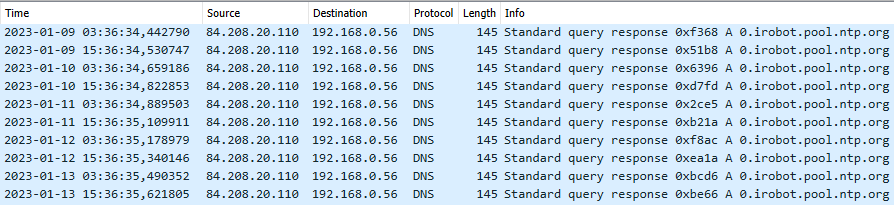
\includegraphics[width=\textwidth]{figures/NTP_wireshark .png}
    \caption{0.irobot.pool.ntp.org DNS resopnse}
    \label{fig:ntp_dns}
\end{figure}

\begin{figure}[H]
    \centering
    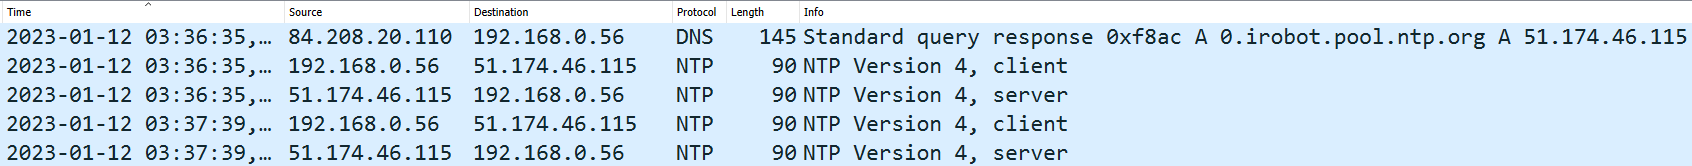
\includegraphics[width=\textwidth]{figures/ntp_dns.png}
    \caption{NTP and DNS realtion}
    \label{fig:ntp_dns}
\end{figure}

\paragraph{DNS} is used by both the robot vacuum cleaner and the access point. The access point is using DNS request to determine if it is connected to Internet or not. This request is for a.root-servers.net, shown in \ref{fig:dns_a-root}. These packegaes can be removed.

\begin{figure}[H]
    \centering
    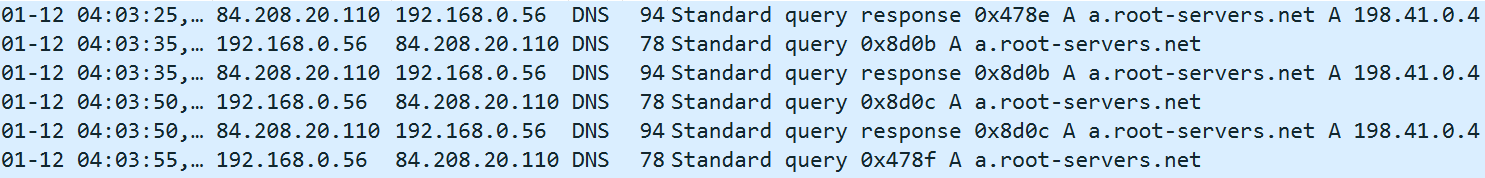
\includegraphics[width=\textwidth]{figures/DNS_a-root.png}
    \caption{Reoccurring DNS Internet test}
    \label{fig:dns_a-root}
\end{figure}

There is two more reocuring DNS reqests created from the TP-link access point. These are requested every three days, most likely to search for updates or upload statistics, and can therefore be excluded.

\begin{itemize}
    \item n-devs-gw.tplinkcloud.com
    \item n-deventry-gw.tplinkcloud.com
\end{itemize}

The Irobot roomba is also requesting these four DNS FQDN once or twice a day: 
\begin{itemize}
    \item 0.irobot.pool.ntp.org
    \item disc-prod.iot.irobotapi.com
    \item unauth1.prod.iot.irobotapi.com
    \item a2uowfjvhio0fa.iot.us-east-1.amazonaws.com
\end{itemize}

After unauth1.prod.iot.irobotapi.com and disc-prod.iot.irobotapi.com, is requested there is a shot traffic flow between the robot vacuum cleaner and the FQDN. If these addresses are opened in a web-browser, this message is prompted \textit{"message":"Missing Authentication Token"}. We are missing the token, which the robot vacuum cleaner authenticate with. 

a2uowfjvhio0fa.iot.us-east-1.amazonaws.com is requested once a day. Each time the robot vacuum cleaner terminates the continuous tcp connections, and opens a new tcp connection to one of the addresses in the response. After the initial tcp handshake it is transferred a lot of data to the new corresponding irobot cloud, before is resumes to what looks like a tcp keep-alive. All these requests are reoccurring and can be excluded from event traffic. 

\subsection{TCP traffic}
Based on the traffic capture it looks like the vacuum cleaner is using tcp to communicate with the cloud service. Since the vacuum cleaner is behind a WAN ISP NAT, the communication needs to be initialized from the vacuum cleaner, and the connection to be held open by continuous traffic flow. This flow is shown in \ref{fig:tcp_keep-alive}. The larges package send in this keep-alive flow is 97 bytes, it is reasonable to assume that all traffic carrying event data will be more then 97 bytes. All tcp packages less then 97 bytes can therefore be excluded. 

\begin{figure}[H]
    \centering
    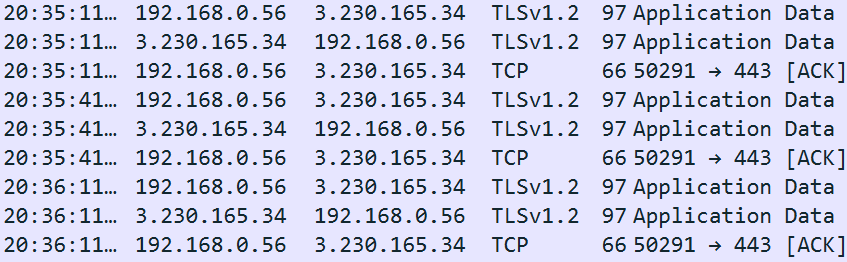
\includegraphics[width=\textwidth]{figures/tcp_keep-alive.png}
    \caption{Reoccurring DNS Internet test}
    \label{fig:tcp_keep-alive}
\end{figure}

\subsection{Data processing results}
The result on this section is a base filter used to exclude all irrelevant data in the event capturing files. From the abow subsections, all DHCP , ARP and NTP can be excluded. The dns request to a.root-servers.net can be handled by the same filter as the tcp keep-alive since both request and response is less then 98 bytes. The base filter will therefor be:
\\
\textit{!ntp \&\& !dhcp \&\& !arp \&\& frame.len > 97}
\\
Some of the other reoccurring DNS requests and data correspondence could still be included, but can more easily be identified. When the filter is applied to the standby capture file, only 0,8 percent of the traffic is left. This makes the manual rule detection process much more efficient. 

\section{Data Analysis}
In this section the entire analysis process for each individual event will be presented separately. In the last subsection there will be a summary and comparison on the different signatures that is found. The process for each event is shown in \ref{fig:dataanalysisprocess}

\begin{figure}[H]
    \centering
    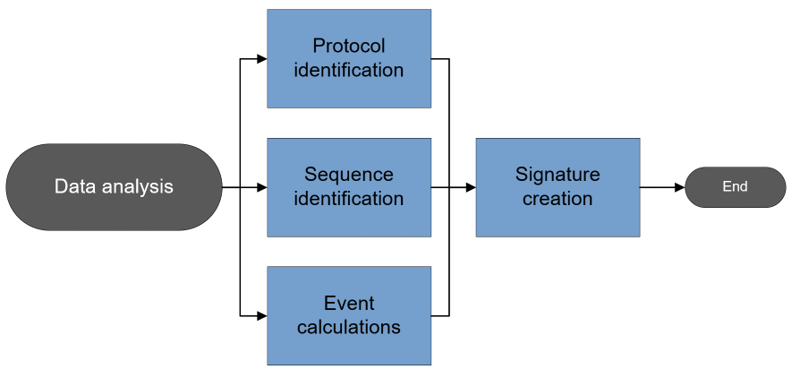
\includegraphics[width=\textwidth]{figures/data-analysis-process.png}
    \caption{Data Analysis Process}
    \label{fig:dataanalysisprocess}
\end{figure}



\subsection{Data analysis for scheduled cleaning}
The overall characteristics for this event is shown in \ref{tab:scoverall} and \ref{tab:scoverallDRA}. As presented the average and the standard deviation within the different environments is small. This supports the hypothesis that is is sufficient with 20 captured events to perform further analysis.

\begin{table}[H]
\centering
\caption{Scheduled cleaning, overall statistics Oslo smart home}
\label{tab:scoverall}
\begin{tabular}{|l|l|l|}
\hline
\textbf{Event} & \textbf{Number of pkt} & \textbf{Total bytes sent} \\ \hline
Event 1        & 2541                   & 3669941                   \\ \hline
Event 2        & 2633                   & 3678959                   \\ \hline
Event 3        & 2622                   & 3660004                   \\ \hline
Event 4        & 2524                   & 3629262                   \\ \hline
Event 5        & 2627                   & 3658515                   \\ \hline
Event 6        & 2608                   & 3729110                   \\ \hline
Event 7        & 2596                   & 3645238                   \\ \hline
Event 8        & 2655                   & 3685536                   \\ \hline
Event 9        & 2573                   & 3713211                   \\ \hline
Event 10       & 2636                   & 3768883                   \\ \hline
Average        & 2601.5                 & 3683865.9                 \\ \hline
\end{tabular}
\end{table}

\begin{table}[H]
\centering
\caption{Scheduled cleaning, overall statistics Drammen}
\label{tab:scoverallDRA}
\begin{tabular}{|l|l|l|}
\hline
\textbf{Event} & \textbf{Number of pkt} & \textbf{Total bytes sent} \\ \hline
Event 1        & 996                    & 1354755                   \\ \hline
Event 2        & 1052                   & 1422052                   \\ \hline
Event 3        & 1150                   & 1592566                   \\ \hline
Event 4        & 1317                   & 1650499                   \\ \hline
Event 5        & 1166                   & 1570805                   \\ \hline
Event 6        & 1179                   & 1612050                   \\ \hline
Event 7        & 1160                   & 1582275                   \\ \hline
Event 8        & 1177                   & 1610090                   \\ \hline
Event 9        & 1205                   & 1634883                   \\ \hline
Event 10       & 1170                   & 1590726                   \\ \hline
Average        & 1157.2                 & 1562070.1                 \\ \hline
\end{tabular}
\end{table}

In \ref{fig:Sc-graph}, the overall traffic flow is displayed. The traffic flow is consistanse for all the captured events, and the large spike of traffic is the session between the vacuum cleaner and S3.amasoneaws.com. There is also a increase in generated traffic at the start of the event, but this is 
deafened by the large upload traffic after finished cleaning.
\begin{figure}[H]
    \centering
    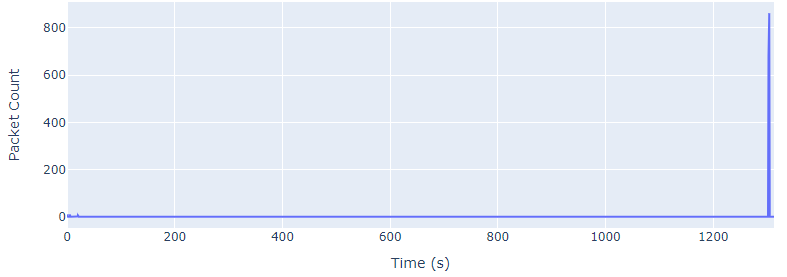
\includegraphics[width=\textwidth]{figures/SC-graph.png}
    \caption{Scheduled clean event 2}
    \label{fig:Sc-graph}
\end{figure}

\subsubsection{Protocol identification}
In scheduled cleaning there is an average protocol distribution according to \ref{tab:scanalysisdist}, this is after the base filter created in data processing is applied. The two UDP packages is DNS response for FQDN:

\begin{itemize}
    \item 0550315.ingest.sentry.io
    \item S3.amasoneaws.com
\end{itemize}

\begin{table}[H]
\centering
\caption{Protocol Statistics Scheduled cleaning}
\label{tab:scanalysisdist}
\begin{tabular}{|c|c|}
\hline
\textbf{Transport protocol} & \textbf{Percentage} \\ \hline
UDP                         & 0,2                 \\ \hline
TCP                         & 99,8                \\ \hline
\end{tabular}
\end{table}

After the cleaning is done, there is two new sessions established. First a session to \textit{0550315.ingest.sentry.io} where the vacuum cleaner is transferring some data. When this session is closed it opens a session to \textit{s3.amazoneaws.com}, where there is sent large amounts of traffic, before the session is closed. Both sessions are established and teared down within a minute after the cleaning is done. This is most likely two different update services where \textit{s3.amazoneaws.com} is where sensed information is uploaded and processed after clenaing.
 
\subsubsection{Traffic sequence}
In the sequence identification we will use the same method as the researchers in \cite{pingpong}. All traffic has the smart home wan address as source or destination due to the infrastructure design. We extract the first 20 bytes of the packet sequence to try to identify a common sequence for all Scheduled cleaning events. Only the first bytes are examined because that is where the event is triggered. In \ref{tab:sclengthseq}, the 20 first bytes of each event is presented. The horizontal values are packet packet lengths, where notation 's' and 'd' notations are WAN address source and destination.  
For this event we can see that the traffic generated by the vacuum cleaner is following a pattern: 
\\
\textit{[176, 173, 179, 443, 177]}, + - 15 bytes on all values 
\\
\textit{[176, 443, 179, 443, 177]} + - 5 bytes in all values
\\
The reason for adding + or - 15 and 5 is because the actual value is varies with the deviation of 15 and 5.

\begin{table}[H]
\small
\centering
\caption{Scheduled cleaning, length sequence}
\label{tab:sclengthseq}
\begin{tabular}{|l|l|l|l|l|l|l|l|l|}
\hline
Event 1  & \colorbox{pink}{S 179} & \colorbox{pink}{S 160} & D 346  & \colorbox{pink}{S 175} & \colorbox{pink}{S 482} & D 1142 & \colorbox{pink}{S 179} & \colorbox{pink}{S 441} \\ \hline
Event 2  & \colorbox{pink}{S 175} & \colorbox{pink}{S 482} & D 1142 & \colorbox{pink}{S 179} & \colorbox{pink}{S 442} & D 1102 & \colorbox{pink}{S 179} & \colorbox{pink}{S 448}  \\ \hline
Event 3  & \colorbox{pink}{S 179} & \colorbox{pink}{S 160} & D 346  & \colorbox{pink}{S 175} & \colorbox{pink}{S 482} & D 1142 & \colorbox{pink}{S 179} & \colorbox{pink}{S 442}  \\ \hline
Event 4  & \colorbox{pink}{S 179} & \colorbox{pink}{S 442} & D 1102 & \colorbox{pink}{S 175} & \colorbox{pink}{S 482} & D 1142 & \colorbox{pink}{S 179} & \colorbox{pink}{S 448}  \\ \hline
Event 5  & \colorbox{pink}{S 179} & \colorbox{pink}{S 253} & D 626  & \colorbox{pink}{S 179} & \colorbox{pink}{S 448} & D 1108 & \colorbox{pink}{S 179} & \colorbox{pink}{S 448}  \\ \hline
Event 6  & \colorbox{pink}{S 179} & \colorbox{pink}{S 442} & D 1102 & \colorbox{pink}{S 175} & \colorbox{pink}{S 482} & D 1142 & \colorbox{pink}{S 179} & \colorbox{pink}{S 448}  \\ \hline
Event 7  & \colorbox{pink}{S 179} & \colorbox{pink}{S 160} & D 346  & \colorbox{pink}{S 175} & \colorbox{pink}{S 482} & D 1142 & \colorbox{pink}{S 179} & \colorbox{pink}{S 442}  \\ \hline
Event 8  & \colorbox{pink}{S 179} & \colorbox{pink}{S 160} & D 346  & \colorbox{pink}{S 175} & \colorbox{pink}{S 482} & D 1142 & \colorbox{pink}{S 179} & \colorbox{pink}{S 442}  \\ \hline
Event 9  & \colorbox{pink}{S 179} & \colorbox{pink}{S 160} & D 346  & \colorbox{pink}{S 175} & \colorbox{pink}{S 482} & D 1142 & \colorbox{pink}{S 179} & \colorbox{pink}{S 442}  \\ \hline
Event 10 & \colorbox{pink}{S 175} & \colorbox{pink}{S 482} & D 1142 & \colorbox{pink}{S 179} & \colorbox{pink}{S 442} & D 1102 & \colorbox{pink}{S 179} & \colorbox{pink}{S 448}  \\ \hline
\end{tabular}
\end{table}


\begin{table}[H]
\centering
\caption{ Scheduled cleaning, length sequence Drammen}
\label{tab:SCsequenceDrammen}
\begin{tabular}{|l|l|l|l|l|l|l|l|l|}
\hline
Event 1  & S 175   & S 466 & D 1094 & S 179 & S 442 & D 1102 & S 179 & S 448 \\ \hline
Event 2  & S 175   & S 466 & D 1094 & S 179 & S 442 & D 1102 & S 179 & S 448 \\ \hline
Event 3  & S 175   & S 466 & D 1094 & S 179 & S 442 & D 1102 & S 179 & S 448 \\ \hline
Event 4  & S 175   & S 466 & D 1094 & S 179 & S 442 & D 1102 & S 179 & S 448 \\ \hline
Event 5  & S 175   & S 466 & D 1094 & S 179 & S 442 & D 1102 & S 179 & S 448 \\ \hline
Event 6  & S 175   & S 466 & D 1094 & S 179 & S 442 & D 1102 & S 179 & S 448 \\ \hline
Event 7  & S 175   & S 466 & D 1094 & S 179 & S 442 & D 1102 & S 179 & S 448 \\ \hline
Event 8  & S 175   & S 466 & D 1094 & S 179 & S 442 & D 1102 & S 179 & S 448 \\ \hline
Event 9  & S 172   & S 234 & D 552  & S 175 & S 466 & D 1094 & S 179 & S 448 \\ \hline
Event 10 & S 175   & S 466 & D 1094 & S 179 & S 442 & D 1102 & S 179 & S 448 \\ \hline
\end{tabular}
\end{table}

\subsubsection{Signeture}
The signature for scheduled cleaning event is the present of DNS request for, \textit{0550315.ingest.sentry.io} and \textit{0550315.ingest.sentry.io} and traffic sequence \textit{[176, 173, 179, 443, 177]} or \textit{[176, 443, 179, 443, 177]}.

The identified signature for Schedule cleaning includes the present of two DNS responses and one of the given sequences.  

\begin{itemize}
    \item \textit{0550315.ingest.sentry.io}
    \item \textit{s3.amazoneaws.com}
    \item \textit{[176, 173, 179, 443, 177]} +- 15
    \item \textit{[176, 443, 179, 443, 177]} +- 5
\end{itemize}



%New section Automated cleaning



\subsection{Data analysis for Automated cleaning}
The overall characteristics for this event is shown in \ref{tab:scoverall} and \ref{tab:scoverallDRA}. As presented the average and the standard deviation within the different environments is small. This supports the hypothesis that is is sufficient with 20 captured events to perform further analysis. Event 6 in Drammen is off the other captures. During analysis all identifications for a cleaning event was present, but the upload to the could service was limited. This could be to some disruption in the transaction or the lack of updates for the vacuum cleaner. 

\begin{table}[H]
\centering
\caption{Automated cleaning, overall statistics Oslo}
\label{tab:ACoverallOSL}
\begin{tabular}{|l|l|l|}
\hline
\textbf{Event} & \textbf{Packet number} & \textbf{Total bytes sent} \\ \hline
Event 1        & 2703                   & 3882164                   \\ \hline
Event 2        & 2736                   & 3811206                   \\ \hline
Event 3        & 2659                   & 3818287                   \\ \hline
Event 4        & 2681                   & 3747788                   \\ \hline
Event 5        & 2589                   & 3704329                   \\ \hline
Event 6        & 236                    & 237163                    \\ \hline
Event 7        & 2701                   & 3860634                   \\ \hline
Event 8        & 2631                   & 3770236                   \\ \hline
Event 9        & 2609                   & 3738406                   \\ \hline
Event 10       & 2609                   & 3799896                   \\ \hline
Average        & 2415.4                 & 3437010.9                 \\ \hline
\end{tabular}
\end{table}

\begin{table}[H]
\centering
\caption{Automated cleaning, overall statistics Drammen}
\label{tab:ACoverallDRA}
\begin{tabular}{|l|l|l|}
\hline
\textbf{Event} & \textbf{Packet number} & \textbf{Total bytes sent} \\ \hline
Event 1        & 1074                   & 1443851                   \\ \hline
Event 2        & 1131                   & 1524076                   \\ \hline
Event 3        & 1209                   & 1644223                   \\ \hline
Event 4        & 1207                   & 1641145                   \\ \hline
Event 5        & 1013                   & 1422457                   \\ \hline
Event 6        & 1013                   & 1422457                   \\ \hline
Event 7        & 1220                   & 1726862                   \\ \hline
Event 8        & 1248                   & 1715015                   \\ \hline
Event 9        & 1227                   & 1669154                   \\ \hline
Event 10       & 1456                   & 1838832                   \\ \hline
Average        & 1179.8                 & 1604807.2                 \\ \hline
\end{tabular}
\end{table}

In \ref{fig:Ac-graph}, the overall traffic flow is displayed. The traffic flow is consistence for all the captured events, and the large spike of traffic is the session between the vacuum cleaner and S3.amasoneaws.com. There is also a increase in generated traffic at the start of the event, but this is 
deafened by the large upload traffic after finished cleaning.

\begin{figure}[H]
    \centering
    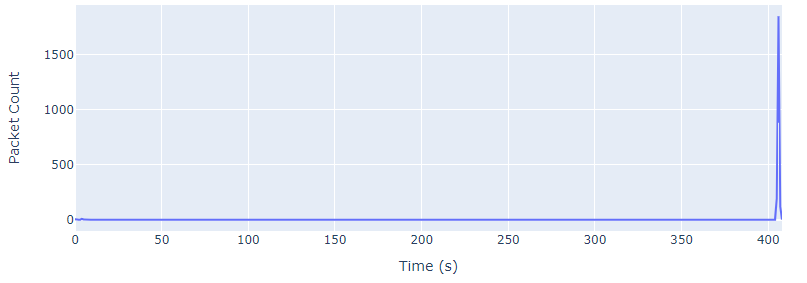
\includegraphics[width=\textwidth]{figures/AC-graph.png}
    \caption{Automated clean event 2 Oslo}
    \label{fig:Ac-graph}
\end{figure}

\subsubsection{Protocol Identification}
In Automated cleaning there is an average protocol distribution according to \ref{tab:acanalysisdist}. All the udp traffic is DNS request, one to each of these FQDNs:

\begin{itemize}
    \item 0550315.ingest.sentry.io
    \item S3.amasoneaws.com
\end{itemize}

\begin{table}[H]
\centering
\caption{Protocol Statistics Automated cleaning}
\label{tab:acanalysisdist}
\begin{tabular}{|c|c|}
\hline
\textbf{Transport protocol} & \textbf{Percentage} \\ \hline
UDP                         & 0,1                 \\ \hline
TCP                         & 99,9                \\ \hline
\end{tabular}
\end{table}

After the cleaning is done, there is two new sessions established. First a session to \textit{0550315.ingest.sentry.io} where the vacuum cleaner is transferring some data. When this session is closed it opens a session to \textit{s3.amazoneaws.com}, where there is sent large amounts of traffic, before the session is closed. Both sessions are established and teared down within a minute after the cleaning is done. This is most likely two different update services where \textit{s3.amazoneaws.com} is where sensed information is uploaded and processed after cleaning.

\subsubsection{Traffic Sequence}
The method in \cite{pingpong} is used manually on the first 20 packet lengths of the event. Inn all 20 events there is a common traffic sequence initiated from the could service, this is \textit{[316, 289]}. these packet lengths dose not occur in the same order, but is received together as a pair. So both \textit{[316, 289]} and \textit{[289, 315]} are valid. The actual packet length also varies with +- 1 byte. 
The following sequence is a response from the vacuum cleaner with packet lengths of \textit{[176, 187]}. Followed by a response from the cloud server with packet length 408 or 409. The identified sequence is therefore: \textit{[316, 289, 176, 187, 409]} or \textit{[289, 316, 176, 187, 409]} +- 1 byte.

\begin{table}[H]
\centering
\caption{Automated cleaning, length sequence Oslo}
\label{tab:ACSequenceOslo}
\begin{tabular}{|l|l|l|l|l|l|l|l|l|}
\hline
Event 1  & D 289 & D 316 & D 316 & S 176 & S 187 & D 409 & D 404 & S 175  \\ \hline
Event 2  & D 510 & S 176 & S 187 & D 409 & D 271 & S 179 & S 440 & D 1100 \\ \hline
Event 3  & D 315 & D 288 & S 176 & S 186 & D 408 & D 271 & D 271 & S 175  \\ \hline
Event 4  & D 315 & D 288 & S 176 & S 186 & D 408 & D 404 & S 175 & S 480  \\ \hline
Event 5  & D 316 & D 289 & S 176 & S 187 & D 409 & D 271 & S 175 & S 405  \\ \hline
Event 6  & D 316 & D 289 & S 176 & S 187 & D 409 & D 271 & S 175 & S 405  \\ \hline
Event 7  & S 172 & S 179 & D 392 & D 315 & D 288 & S 176 & S 186 & D 408  \\ \hline
Event 8  & S 172 & S 179 & D 392 & D 315 & D 288 & S 176 & S 186 & D 408  \\ \hline
Event 9  & D 289 & D 316 & S 176 & S 187 & D 409 & D 271 & S 179 & S 440  \\ \hline
Event 10 & S 172 & S 291 & D 859 & D 288 & D 315 & S 176 & S 186 & D 408  \\ \hline
\end{tabular}
\end{table}


\begin{table}[H]
\centering
\caption{Automated cleaning, length sequence Drammen}
\label{tab:ACSequenceDrammen}
\begin{tabular}{|l|l|l|l|l|l|l|l|l|}
\hline
Event 1  & D 315 & D 288 & S 176 & S 186 & D 408 & D 404 & S 175 & S 425  \\ \hline
Event 2  & D 289 & D 316 & S 176 & S 187 & D 409 & D 404 & S 175 & S 449  \\ \hline
Event 3  & S 172 & S 288 & D 714 & D 316 & D 289 & S 176 & S 187 & D 409  \\ \hline
Event 4  & D 315 & D 288 & S 176 & S 186 & D 408 & D 404 & S 179 & S 439  \\ \hline
Event 5  & D 289 & D 316 & S 176 & S 187 & D 409 & D 404 & S 175 & S 410  \\ \hline
Event 6  & D 289 & D 316 & D 316 & S 176 & S 187 & D 409 & D 404 & S 175  \\ \hline
Event 7  & D 288 & D 315 & S 176 & S 186 & D 408 & D 404 & S 175 & S 449  \\ \hline
Event 8  & D 289 & D 316 & S 297 & D 409 & D 404 & S 179 & S 440 & D 1100 \\ \hline
Event 9  & S 172 & S 233 & D 551 & D 315 & D 288 & S 176 & S 186 & D 408  \\ \hline
Event 10 & D 289 & D 316 & S 176 & S 187 & D 409 & D 404 & S 179 & S 440  \\ \hline
\end{tabular}
\end{table}

\subsubsection{Signature}
The identified signature for Automated cleaning includes the present of two DNS responses and one of the given sequences.  

\begin{itemize}
    \item \textit{0550315.ingest.sentry.io}
    \item \textit{s3.amazoneaws.com}
    \item \textit{[316, 289, 176, 187, 409]} +- 1
    \item \textit{[289, 316, 176, 187, 409]} +- 1
\end{itemize}


\subsection{Data Analysis for Application Triggered Cleaning}
The overall characteristics for this event is shown in \ref{tab:TCoverallOSL} and \ref{tab:TCoverallDRA}. As presented the average and the standard deviation within the different environments is small. This supports the hypothesis that is is sufficient with 20 captured events to perform further analysis.

\begin{table}[H]
\centering
\caption{Application triggered cleaning, overall statistics Oslo}
\label{tab:TCoverallOSL}
\begin{tabular}{|l|l|l|}
\hline
\textbf{Event} & \textbf{Packet number} & \textbf{Total bytes sent} \\ \hline
Event 1        & 2667                   & 3732218                   \\ \hline
Event 2        & 2686                   & 3730748                   \\ \hline
Event 3        & 2656                   & 3710958                   \\ \hline
Event 4        & 3065                   & 4365510                   \\ \hline
Event 5        & 2880                   & 4076534                   \\ \hline
Event 6        & 2633                   & 3771269                   \\ \hline
Event 7        & 2661                   & 3786648                   \\ \hline
Event 8        & 2647                   & 3798184                   \\ \hline
Event 9        & 2729                   & 3798630                   \\ \hline
Event 10       & 2639                   & 3786194                   \\ \hline
Average        & 2726.3                 & 3855689.3                 \\ \hline
\end{tabular}
\end{table}

\begin{table}[H]
\centering
\caption{Application triggered cleaning, overall statistics Drammen}
\label{tab:TCoverallDRA}
\begin{tabular}{|l|l|l|}
\hline
\textbf{Event} & \textbf{Packet number} & \textbf{Total bytes sent} \\ \hline
Event 1        & 708                    & 802488                    \\ \hline
Event 2        & 724                    & 945100                    \\ \hline
Event 3        & 740                    & 956470                    \\ \hline
Event 4        & 809                    & 1071613                   \\ \hline
Event 5        & 824                    & 1088836                   \\ \hline
Event 6        & 869                    & 1157323                   \\ \hline
Event 7        & 855                    & 1144086                   \\ \hline
Event 8        & 929                    & 1248783                   \\ \hline
Event 9        & 988                    & 1321061                   \\ \hline
Event 10       & 983                    & 1339631                   \\ \hline
Average        & 842.9                  & 1107539.1                 \\ \hline
\end{tabular}
\end{table}

In \ref{fig:Tc-graph}, the overall traffic flow is displayed. The traffic flow is consistence for all the captured events, and the large spike of traffic is the session between the vacuum cleaner and S3.amasoneaws.com. There is also a increase in generated traffic at the start of the event, but this is 
deafened by the large upload traffic after finished cleaning.

\begin{figure}[H]
    \centering
    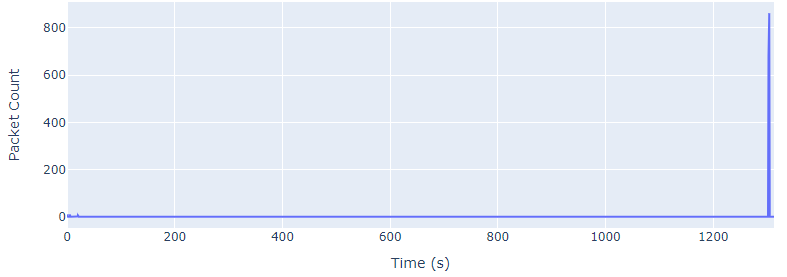
\includegraphics[width=\textwidth]{figures/TC-graph.png}
    \caption{Automated clean event 2 Oslo}
    \label{fig:Tc-graph}
\end{figure}

\subsubsection{Protocol Identification}
In Automated cleaning there is an average protocol distribution according to \ref{tab:tcanalysisdist}. All the udp traffic is DNS request, one to each of these FQDNs:
\\
figure
\\



After the cleaning is done, there is two new sessions established. First a session to \textit{0550315.ingest.sentry.io} where the vacuum cleaner is transferring some data. When this session is closed it opens a session to \textit{s3.amazoneaws.com}, where there is sent large amounts of traffic, before the session is closed. Both sessions are established and teared down within a minute after the cleaning is done. This is most likely two different update services where \textit{s3.amazoneaws.com} is where sensed information is uploaded and processed after cleaning.

\subsubsection{Traffic sequence}
The method in [pingpong] is used manually on the first 20 packet lengths of the
event.All events has a common sequence initiated from the cloud service, \textit{[209, 289, 316]} where the two last packets can be in mixed order. The vacuum cleaner then responds with two packets with length \textit{176, 187}, before the could service responds with a package with length \textit{409 or 408}. The entire packet sequence is then \textit{[316, 289, 176, 187, 409] or [289, 316, 176, 187, 409]
}

\begin{table}[H]
\centering
\caption{Application triggered cleaning, length sequence Oslo}
\label{tab:ACSequenceOslo}
\begin{tabular}{|l|l|l|l|l|l|l|l|l|}
\hline
Event 1  & D 208 & D 288 & D 315 & S 176  & S 186  & D 408 & S 176 & S 1285 \\ \hline
Event 2  & S 179 & S 160 & D 346 & D 209  & D 289  & D 316 & S 176 & S 187  \\ \hline
Event 3  & D 208 & D 289 & D 316 & S 176  & S 187  & D 409 & S 176 & S 1514 \\ \hline
Event 4  & S 179 & S 160 & D 346 & D 208  & D 288  & D 315 & S 176 & S 186  \\ \hline
Event 5  & S 179 & S 160 & D 346 & D 208  & D 288  & D 315 & S 176 & S 186  \\ \hline
Event 6  & S 179 & S 160 & D 346 & S 172  & S 233  & D 551 & D 209 & D 289  \\ \hline
Event 7  & D 209 & D 315 & D 288 & S 176  & S 186  & D 408 & S 176 & S 1201 \\ \hline
Event 8  & S 179 & S 160 & D 346 & D 209  & D 316  & D 289 & S 176 & S 187  \\ \hline
Event 9  & D 209 & D 510 & S 176 & S 1201 & S 176  & S 187 & D 409 & D 555  \\ \hline
Event 10 & D 209 & D 288 & D 315 & S 176  & S 1201 & S 176 & S 186 & D 408  \\ \hline
\end{tabular}
\end{table}

\begin{table}[H]
\centering
\caption{Application triggered cleaning, length sequence Drammen}
\label{tab:ACSequenceDrammen}
\begin{tabular}{|l|l|l|l|l|l|l|l|l|}
\hline
Event 1  & D 209 & D 315 & D 288 & S 176 & S 186  & D 408 & S 176 & S 949  \\ \hline
Event 2  & D 208 & D 289 & D 316 & S 176 & S 187  & D 409 & S 176 & S 1514 \\ \hline
Event 3  & D 209 & D 316 & D 289 & S 176 & S 187  & D 409 & S 176 & S 1514 \\ \hline
Event 4  & D 209 & D 288 & D 315 & S 176 & S 1085 & S 176 & S 186 & D 408  \\ \hline
Event 5  & S 179 & S 160 & D 346 & D 209 & D 316  & D 289 & S 176 & S 1514 \\ \hline
Event 6  & S 172 & S 179 & D 392 & D 208 & D 315  & D 288 & S 176 & S 186  \\ \hline
Event 7  & D 207 & D 289 & D 316 & S 176 & S 187  & D 409 & S 176 & S 1514 \\ \hline
Event 8  & D 207 & D 315 & D 288 & S 176 & S 186  & D 408 & S 176 & S 1514 \\ \hline
Event 9  & D 208 & D 315 & D 288 & S 176 & S 985  & S 176 & S 186 & D 408  \\ \hline
Event 10 & D 208 & D 315 & D 288 & S 176 & S 186  & D 408 & S 176 & S 1514 \\ \hline
\end{tabular}
\end{table}

\subsubsection{Signature}
The identified signature for Application triggered cleaning includes the present of two DNS
responses and one of the given sequences.
• 0550315.ingest.sentry.io
• s3.amazoneaws.com
• [209, 316, 289, 176, 187, 409] +- 1
• [209, 289, 316, 176, 187, 409] +- 1





%new event









\subsection{Data Analysis for Physical triggered cleaning}

\begin{table}[H]
\centering
\caption{Physical triggered cleaning, overall statistics Oslo}
\label{tab:PCoverallOSL}
\begin{tabular}{|l|l|l|}
\hline
\textbf{Event} & \textbf{Packet number} & \textbf{Total bytes sent} \\ \hline
Event 1        & 2791                   & 3965147                   \\ \hline
Event 2        & 3180                   & 4357126                   \\ \hline
Event 3        & 2926                   & 4033946                   \\ \hline
Event 4        & 2872                   & 4112516                   \\ \hline
Event 5        & 2944                   & 4209443                   \\ \hline
Event 6        & 2984                   & 4122412                   \\ \hline
Event 7        & 2925                   & 4160462                   \\ \hline
Event 8        & 2869                   & 4100166                   \\ \hline
Event 9        & 2918                   & 4227626                   \\ \hline
Event 10       & 2768                   & 3957559                   \\ \hline
Average        & 2917.7                 & 4124640.3                 \\ \hline
\end{tabular}
\end{table}

\begin{table}[H]
\centering
\caption{Physical triggered cleaning, overall statistics Drammen}
\label{tab:PCoverallDRA}
\begin{tabular}{|l|l|l|}
\hline
\textbf{Event} & \textbf{Packet number} & \textbf{Total bytes sent} \\ \hline
Event 1        & 1078                   & 1481677                   \\ \hline
Event 2        & 1087                   & 1484930                   \\ \hline
Event 3        & 1125                   & 1520872                   \\ \hline
Event 4        & 1088                   & 1517429                   \\ \hline
Event 5        & 1150                   & 1555605                   \\ \hline
Event 6        & 1086                   & 1507084                   \\ \hline
Event 7        & 1092                   & 1501894                   \\ \hline
Event 8        & 1115                   & 1510971                   \\ \hline
Event 9        & 1098                   & 1485863                   \\ \hline
Event 10       & 1100                   & 1492331                   \\ \hline
Average        & 1101.9                 & 1505865.6                 \\ \hline
\end{tabular}
\end{table}

In \ref{fig:Pc-graph}, the overall traffic flow is displayed. the large spike of traffic is the session between the vacuum cleaner and S3.amasoneaws.com.
\begin{figure}[H]
    \centering
    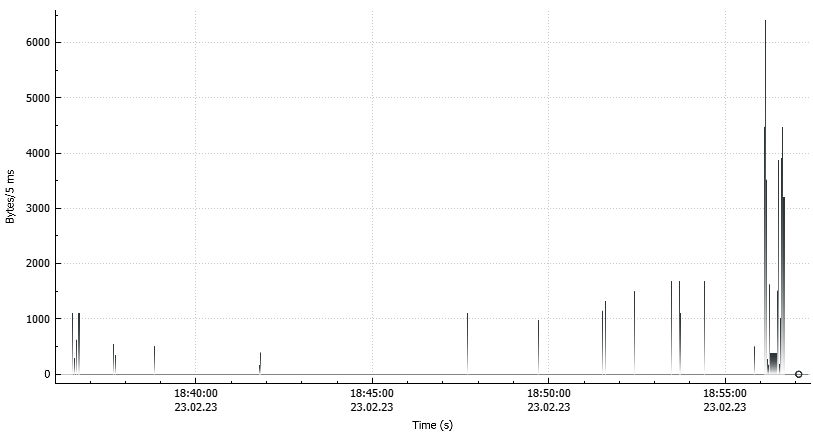
\includegraphics[width=\textwidth]{figures/PC-graph.png}
    \caption{Automated clean event 2 Oslo}
    \label{fig:Pc-graph}
\end{figure}

\subsubsection{Protocol Identification}

\subsubsection{Traffic sequence}

\begin{table}[H]
\centering
\caption{Physical triggered cleaning, length sequence Oslo}
\label{tab:PCSequenceOslo}
\begin{tabular}{|l|l|l|l|l|l|l|l|l|}
\hline
Event 1  & S 179 & S 440 & D 1100 & S 179 & S 446 & D 1106 & S 176 & S 475 \\ \hline
Event 2  & S 179 & S 159 & D 345  & S 179 & S 446 & D 1106 & S 176 & S 290 \\ \hline
Event 3  & S 179 & S 160 & D 346  & S 179 & S 440 & D 1100 & S 179 & S 446 \\ \hline
Event 4  & S 179 & S 160 & D 346  & S 179 & S 440 & D 1100 & S 179 & S 446 \\ \hline
Event 5  & S 179 & S 440 & D 1100 & S 179 & S 446 & D 1106 & S 176 & S 290 \\ \hline
Event 6  & S 179 & S 440 & D 1100 & S 179 & S 446 & D 1106 & S 175 & S 369 \\ \hline
Event 7  & S 172 & S 179 & D 392  & S 179 & S 446 & D 1106 & S 176 & S 290 \\ \hline
Event 8  & S 179 & S 440 & D 1100 & S 179 & S 446 & D 1106 & S 176 & S 290 \\ \hline
Event 9  & S 179 & S 440 & D 1100 & S 179 & S 446 & D 1106 & S 176 & S 290 \\ \hline
Event 10 & S 179 & S 159 & D 345  & S 179 & S 440 & D 1100 & S 179 & S 446 \\ \hline
\end{tabular}
\end{table}

\begin{table}[H]
\centering
\caption{Physical triggered cleaning, length sequence Drammen}
\label{tab:PCSequenceDrammen}
\begin{tabular}{|l|l|l|l|l|l|l|l|l|}
\hline
Event 1  & S 175 & S 314 & D 745  & S 179 & S 447 & D 1107 & S 179 & S 447 \\ \hline
Event 2  & S 179 & S 446 & D 1106 & S 176 & S 290 & S 175  & S 338 & D 809 \\ \hline
Event 3  & S 179 & S 440 & D 1100 & S 179 & S 446 & D 1106 & S 176 & S 290 \\ \hline
Event 4  & S 179 & S 159 & D 345  & S 179 & S 440 & D 1100 & S 179 & S 446 \\ \hline
Event 5  & S 179 & S 439 & D 1099 & S 179 & S 445 & D 1105 & S 175 & S 314 \\ \hline
Event 6  & S 179 & S 439 & D 1099 & S 179 & S 445 & D 1105 & S 175 & S 314 \\ \hline
Event 7  & S 179 & S 160 & D 346  & S 179 & S 439 & D 1099 & S 179 & S 445 \\ \hline
Event 8  & S 172 & S 233 & D 551  & S 179 & S 439 & D 1099 & S 179 & S 445 \\ \hline
Event 9  & S 179 & S 440 & D 1100 & S 179 & S 446 & D 1106 & S 175 & S 338 \\ \hline
Event 10 & S 179 & S 440 & D 1100 & S 179 & S 446 & D 1106 & S 175 & S 338 \\ \hline
\end{tabular}
\end{table}

\subsubsection{Signature}


\subsection{Data Analysis for Application Start}

\begin{table}[H]
\centering
\caption{Application start, overall statistics Oslo}
\label{tab:ASoverallOslo}
\begin{tabular}{|l|l|l|}
\hline
\textbf{Event} & \textbf{Packet number} & \textbf{Total bytes sent} \\ \hline
Event 1        & 11                     & 5202                      \\ \hline
Event 2        & 22                     & 8698                      \\ \hline
Event 3        & 20                     & 8644                      \\ \hline
Event 4        & 17                     & 7135                      \\ \hline
Event 5        & 20                     & 8580                      \\ \hline
Event 6        & 20                     & 8608                      \\ \hline
Event 7        & 20                     & 9213                      \\ \hline
Event 8        & 23                     & 9527                      \\ \hline
Event 9        & 20                     & 8730                      \\ \hline
Event 10       & 19                     & 8877                      \\ \hline
Average        & 19.2                   & 8321.4                    \\ \hline
\end{tabular}
\end{table}

\begin{table}[H]
\centering
\caption{Application start, overall statistics Drammen}
\label{tab:ASoverallDRA}
\begin{tabular}{|l|l|l|}
\hline
\textbf{Event} & \textbf{Packet number} & \textbf{Total bytes sent} \\ \hline
Event 1        & 30                     & 20875                     \\ \hline
Event 2        & 26                     & 19568                     \\ \hline
Event 3        & 8                      & 2655                      \\ \hline
Event 4        & 8                      & 2659                      \\ \hline
Event 5        & 26                     & 19561                     \\ \hline
Event 6        & 34                     & 21897                     \\ \hline
Event 7        & 29                     & 20222                     \\ \hline
Event 8        & 25                     & 19468                     \\ \hline
Event 9        & 33                     & 21744                     \\ \hline
Event 10       & 26                     & 19570                     \\ \hline
Average        & 24,5                   & 16821.9                   \\ \hline
\end{tabular}
\end{table}

\subsubsection{Protocol Identification}

\subsubsection{Traffic sequence}

\begin{table}[H]
\centering
\caption{Application start, length sequence Oslo}
\label{tab:ASSequenceOslo}
\begin{tabular}{|l|l|l|l|l|l|l|l|l|}
\hline
Event 1  & D 209 & D 315 & D 288 & S 296  & D 408  & S 176 & S 1053 & D 1514 \\ \hline
Event 2  & D 208 & D 316 & D 289 & S 176  & S 187  & D 409 & S 176  & S 1052 \\ \hline
Event 3  & D 208 & D 537 & S 176 & S 186  & D 408  & S 176 & S 1052 & D 1514 \\ \hline
Event 4  & S 179 & S 160 & D 346 & D 208  & D 289  & D 316 & S 176  & S 187  \\ \hline
Event 5  & D 209 & D 315 & D 288 & S 176  & S 186  & D 408 & S 176  & S 1053 \\ \hline
Event 6  & D 205 & D 289 & D 316 & S 176  & S 1046 & S 176 & S 187  & D 409  \\ \hline
Event 7  & D 207 & D 315 & D 288 & S 176  & S 186  & D 408 & S 176  & S 1051 \\ \hline
Event 8  & S 179 & S 159 & D 345 & D 207  & D 289  & D 316 & S 176  & S 187  \\ \hline
Event 9  & D 207 & D 508 & S 176 & S 1050 & S 176  & S 186 & D 408  & D 1514 \\ \hline
Event 10 & D 208 & D 316 & D 289 & S 176  & S 1052 & S 176 & S 187  & D 409  \\ \hline
\end{tabular}
\end{table}

\begin{table}[H]
\centering
\caption{Application start, length sequence Drammen}
\label{tab:ASSequenceDrammen}
\begin{tabular}{|l|l|l|l|l|l|l|l|l|}
\hline
Event 1  & D 209 & D 288 & D 315 & S 296 & D 408  & S 176 & S 1514 & S 376  \\ \hline
Event 2  & D 209 & D 289 & D 316 & S 176 & S 187  & D 409 & S 176  & S 1514 \\ \hline
Event 3  & D 209 & D 315 & D 288 & S 176 & S 186  & D 408 & S 176  & S 1514 \\ \hline
Event 4  & D 209 & D 289 & D 316 & S 176 & S 1514 & S 159 & S 176  & S 187  \\ \hline
Event 5  & S 172 & S 179 & D 392 & D 208 & D 315  & D 288 & S 176  & S 186  \\ \hline
Event 6  & D 208 & D 289 & D 316 & S 176 & S 187  & D 409 & S 176  & S 1514 \\ \hline
Event 7  & D 208 & D 288 & D 315 & S 176 & S 1361 & S 176 & S 186  & D 408  \\ \hline
Event 8  & D 208 & D 289 & D 316 & S 176 & S 187  & D 409 & S 176  & S 1514 \\ \hline
Event 9  & D 208 & D 288 & D 315 & S 176 & S 1514 & S 126 & S 176  & S 186  \\ \hline
Event 10 & D 208 & D 289 & D 316 & S 176 & S 187  & D 409 & S 176  & S 1389 \\ \hline
\end{tabular}
\end{table}

\subsubsection{Signature}


\subsection{Data Analysis for Bin Remove}

\begin{table}[H]
\centering
\caption{Bin remove, overall statistics Oslo}
\label{tab:BRoverallOslo}
\begin{tabular}{|l|l|l|}
\hline
\textbf{Event} & \textbf{Packet number} & \textbf{Total bytes sent} \\ \hline
Event 1        & 6                      & 2512                      \\ \hline
Event 2        & 15                     & 5765                      \\ \hline
Event 3        & 12                     & 4366                      \\ \hline
Event 4        & 15                     & 7869                      \\ \hline
Event 5        & 12                     & 5022                      \\ \hline
Event 6        & 17                     & 8426                      \\ \hline
Event 7        & 18                     & 8492                      \\ \hline
Event 8        & 12                     & 5022                      \\ \hline
Event 9        & 11                     & 4956                      \\ \hline
Event 10       & 12                     & 5022                      \\ \hline
Average        & 13                     & 5745.2                    \\ \hline
\end{tabular}
\end{table}


\begin{table}[H]
\centering
\caption{Bin remove, overall statistics Drammen }
\label{tab:BRoverallDRA}
\begin{tabular}{|l|l|l|}
\hline
\textbf{Event} & \textbf{Packet number} & \textbf{Total bytes sent} \\ \hline
Event 1        & 23                     & 8610                      \\ \hline
Event 2        & 24                     & 10149                     \\ \hline
Event 3        & 9                      & 4407                      \\ \hline
Event 4        & 12                     & 5022                      \\ \hline
Event 5        & 8                      & 4333                      \\ \hline
Event 6        & 9                      & 4399                      \\ \hline
Event 7        & 17                     & 6595                      \\ \hline
Event 8        & 9                      & 4399                      \\ \hline
Event 9        & 15                     & 7869                      \\ \hline
Event 10       & 12                     & 5022                      \\ \hline
Average        & 13,8                   & 6080.5                    \\ \hline
\end{tabular}
\end{table}

\subsubsection{Protocol Identification}

\subsubsection{Traffic sequence}

\begin{table}[H]
\centering
\caption{Bin removal, length sequence Oslo}
\label{tab:BRSquenceOslo}
\begin{tabular}{|l|l|l|l|l|l|l|l|l|}
\hline
Event 1  & S 179   & S 450  & D 1110 & S 179  & S 186  & D 410  & S 179 & S 450 \\ \hline
Event 2  & S   187 & D 411  & S 179  & S 448  & D 1108 & S 179  & S 186 & D 410 \\ \hline
Event 3  & S   179 & S 187  & D 411  & S 179  & S 450  & D 1110 & S 179 & S 450 \\ \hline
Event 4  & S   492 & D 1222 & S 179  & S 450  & D 1110 & S 179  & S 186 & D 410 \\ \hline
Event 5  & S   187 & D 411  & S 179  & S 448  & D 1108 & S 179  & S 186 & D 410 \\ \hline
Event 6  & S 603   & D 1220 & S 179  & S 448  & D 1108 & S 179  & S 186 & D 410 \\ \hline
Event 7  & S   490 & D 1220 & S 179  & S 448  & D 1108 & S 179  & S 186 & D 410 \\ \hline
Event 8  & D   411 & S 179  & S 448  & D 1108 & S 179  & S 186  & D 410 & S 172 \\ \hline
Event 9  & S   490 & D 1220 & S 179  & S 448  & D 1108 & S 179  & S 186 & D 410 \\ \hline
Event 10 & S   448 & D 1108 & S 179  & S 448  & D 1108 & S 179  & S 186 & D 410 \\ \hline
\end{tabular}
\end{table}


\begin{table}[H]
\centering
\caption{Bin removal, length sequence Drammen}
\label{tab:BRSquenceDrammen}
\begin{tabular}{|l|l|l|l|l|l|l|l|l|}
\hline
Event 1  & S 179   & S 448  & D 1108 & S 179 & S 187  & D 411 &       &       \\ \hline
Event 2  & S   187 & D 411  & S 179  & S 448 & D 1108 & S 179 & S 186 & D 410 \\ \hline
Event 3  & S   187 & D 411  & S 179  & S 448 & D 1108 & S 179 & S 186 & D 410 \\ \hline
Event 4  & S   179 & D 392  & S 179  & S 448 & D 1108 & S 179 & S 186 & D 410 \\ \hline
Event 5  & S   448 & D 1108 & S 179  & S 187 & D 411  & S 172 & S 234 & D 552 \\ \hline
Event 6  & S 179   & S 448  & D 1108 & S 179 & S 187  & D 411 & S 179 & S 448 \\ \hline
Event 7  & S   187 & D 411  & S 179  & S 448 & D 1108 & S 179 & S 186 & D 410 \\ \hline
Event 8  & S   448 & D 1108 & S 179  & S 448 & D 1108 & S 179 & S 186 & D 410 \\ \hline
Event 9  & S   448 & D 1108 & S 179  & S 448 & D 1108 & S 179 & S 186 & D 410 \\ \hline
Event 10 & S   187 & D 411  & S 179  & S 448 & D 1108 & S 179 & S 186 & D 410 \\ \hline
\end{tabular}
\end{table}
\subsubsection{Signature}


\subsection{Signature comparison}
All cleaning events has the same DNS signature